\begin{table}[H]
\caption{Simbol Standar \emph{Flowchart} Program}

\centering{}(Sumber: \citealp{chaudhuri2020flowchart})
\end{table}

\vspace{-25pt}

\begin{longtable}[c]{|>{\centering}m{4cm}|>{\raggedright}m{9.5cm}|}
\hline 
\textbf{Simbol} & \centering{}\textbf{Keterangan}\tabularnewline
\hline 
\endfirsthead
\hline 
\textbf{Simbol} & \centering{}\textbf{Keterangan}\tabularnewline
\hline 
\endhead
\hline 
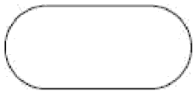
\includegraphics[totalheight=1.3cm]{images/flow_terminal} & Terminal:

Digunakan untuk menunjukkan awal dan akhir dari rangkaian proses yang
berhubungan dengan komputer.\tabularnewline
\hline 
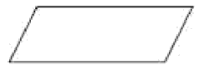
\includegraphics[totalheight=1cm]{images/flow_io} & \emph{Input/Output} (Masukan/Keluaran):

Digunakan untuk menunjukkan operasi \emph{input/output} apa pun.\tabularnewline
\hline 
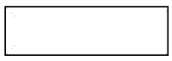
\includegraphics[totalheight=1cm]{images/flow_proc} & Pemrosesan Komputer (\emph{Computer Processing}):

Digunakan untuk menunjukkan pemrosesan apa pun yang dilakukan oleh
sistem komputer.\tabularnewline
\hline 
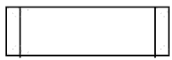
\includegraphics[totalheight=1cm]{images/flow_predproc} & Pemrosesan Tertentu (\emph{Predefined processing}):

Digunakan untuk menunjukkan proses apa pun yang tidak didefinisikan
secara khusus dalam \emph{flowchart}.\tabularnewline
\hline 

\includegraphics[totalheight=1cm]{images/flow_comm} & Komentar (\emph{Comment}):

Digunakan untuk menulis pernyataan penjelasan yang diperlukan untuk
memperjelas sesuatu.\tabularnewline
\hline 
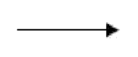
\includegraphics[totalheight=1.5cm]{images/flow_fl} & Garis Alir (\emph{Flow line}):

Digunakan untuk menghubungkan simbol-simbol \emph{flowchart}.\tabularnewline
\hline 
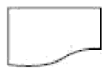
\includegraphics[totalheight=1.5cm]{images/flow_docio} & Masukan/Keluaran Dokumen (\emph{Document Input/Output}):

Digunakan ketika \emph{input} berasal dari dokumen dan \emph{output}
menuju ke dokumen.\tabularnewline
\hline 
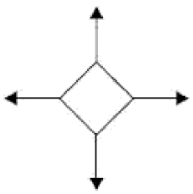
\includegraphics[totalheight=1.8cm]{images/flow_deci} & Keputusan (\emph{Decision}):

Digunakan untuk menunjukkan titik mana pun dalam proses di mana keputusan
harus dibuat untuk menentukan tindakan selanjutnya.\tabularnewline
\hline 
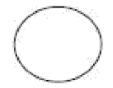
\includegraphics[totalheight=1.7cm]{images/flow_oncon} & Penghubung Halaman (\emph{On-page Connector}):

Digunakan untuk menghubungkan bagian-bagian \emph{flowchart} yang
dilanjutkan pada halaman yang sama.\tabularnewline
\hline 
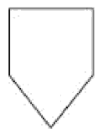
\includegraphics[totalheight=1.9cm]{images/flow_offcon} & Penghubung Antar-Halaman (\emph{Off-page Connector}):

Digunakan untuk menghubungkan bagian-bagian \emph{flowchart} yang
dilanjutkan ke halaman yang terpisah.\tabularnewline
\hline 
\end{longtable}